% Template for the write-up. Do not edit numbers here: every double-angle-bracket placeholder is filled
% from results/*.csv by report/build_report.py, which then compiles report.tex.
\documentclass[10pt,a4paper]{article}
\usepackage[T1]{fontenc}
\usepackage{lmodern}
\usepackage[margin=1.9cm]{geometry}
\usepackage{amsmath,amssymb}
\usepackage{booktabs}
\usepackage{graphicx}
\usepackage{xcolor}
\usepackage[hidelinks]{hyperref}
\graphicspath{{../figures/}}
\setlength{\parindent}{0pt}
\setlength{\parskip}{4pt}
\setlength{\abovedisplayskip}{5pt}
\setlength{\belowdisplayskip}{5pt}
\newcommand{\VaR}{\mathrm{VaR}}
% tighter lists and section headings (no enumitem/titlesec needed)
\let\olditemize\itemize
\renewcommand{\itemize}{\olditemize\setlength{\itemsep}{1pt}\setlength{\parskip}{1pt}\setlength{\topsep}{2pt}}
\makeatletter
\renewcommand{\section}{\@startsection{section}{1}{\z@}{-2.2ex plus -0.5ex}{0.8ex}{\normalfont\large\bfseries}}
\makeatother
\setcounter{topnumber}{3}\renewcommand{\topfraction}{0.9}\renewcommand{\textfraction}{0.1}
\renewcommand{\floatpagefraction}{0.8}

\title{\vspace{-1.6cm}\textbf{Volatility clustering, fat tails and Value-at-Risk\\for the Nikkei 225}}
\author{}
\date{\vspace{-1.4cm}\small Gaussian, Merton jump-diffusion and GARCH one-day VaR, trained on 2000--2011 and backtested on 2012--2026}

\begin{document}
\maketitle

\section{Question and data}

\textbf{Question.} Can a one-day Value-at-Risk (VaR) model estimated on 2000--2011 Nikkei 225 data pass standard
coverage and independence backtests on 2012--2026? And which feature of the returns matters more for that: fat tails
(Merton jump-diffusion) or volatility clustering (GARCH)?

\textbf{Data.} Daily closing levels of the Nikkei 225 (Yahoo Finance ticker \texttt{\^{}N225}, auto-adjusted),
downloaded with \texttt{yfinance} on <<download_date>> and stored as \texttt{data/n225.csv}. Prices run from
4 January 2000 to 30 October 2026, giving <<n_full>> daily log returns in percent,
\[
  r_t = 100\,\ln\!\left(P_t / P_{t-1}\right).
\]
The training set is every return before 1 January 2012 (<<n_tr>> days, 5 Jan 2000 -- 30 Dec 2011). The test set is
every return from then on (<<n_te>> days, 4 Jan 2012 -- 30 Oct 2026). Returns are fat-tailed (kurtosis <<kurt_full>>,
skewness $<<skew_full>>$). On the training data the Ljung--Box test finds little autocorrelation in the returns themselves
($p = <<lb_p5>>$ at 5 lags, $<<lb_p10>>$ at 10). It finds very strong autocorrelation in squared returns ($Q = <<lb_q5>>$
at 5 lags, $p < 0.001$ at every lag tested), so volatility clusters.

\section{Methods}

\textbf{Mean forecasts (baseline).} OLS autoregressions with 1--5 lags, fitted with scikit-learn's
\texttt{LinearRegression}. They are refitted every test day on all earlier days (expanding walk-forward, so the forecast
for day $t$ uses data up to $t-1$ only). They are compared with a zero forecast and with the expanding historical mean,
using out-of-sample $R^2$ and a simple $t$-statistic on the daily squared-error difference, without a correction for
autocorrelation.

\textbf{Gaussian.} Returns are i.i.d.\ $\mathcal N(\mu,\sigma^2)$, with maximum-likelihood estimates from the training
data.

\textbf{Merton jump-diffusion.} Returns are i.i.d.\ with $r = \mu + \sigma Z + \sum_{j=1}^{N} J_j$, where
$N \sim \mathrm{Poisson}(\lambda)$ and $J_j \sim \mathcal N(m,\delta^2)$. This gives a Poisson-weighted mixture of
normals, truncated at $K = 10$ jumps:
\[
  f(r) = \sum_{k=0}^{K} \frac{e^{-\lambda}\lambda^{k}}{k!}\;
         \phi\!\left(r;\ \mu + k m,\ \sigma^{2} + k\delta^{2}\right).
\]
I wrote the likelihood by hand and maximised it with scipy's Nelder--Mead from three starting points; all three reach the
same log-likelihood. The two densities are compared out of sample by the daily log-score difference
\[
  d_t = \log f_{\text{Merton}}(r_t) - \log f_{\text{Gauss}}(r_t),
\]
decomposed by $|r_t|$ bucket. A moving-block bootstrap gives a confidence interval for its mean (5{,}000 resamples,
blocks of 10, 20 and 60 days, seed 42).

\textbf{GARCH.} With $\varepsilon_t = r_t - \mu$ ($\mu$ is the training mean), the conditional variance follows
\[
  \sigma_t^{2} = \omega + \bigl(\alpha + \gamma\,\mathbf{1}[\varepsilon_{t-1} < 0]\bigr)\,\varepsilon_{t-1}^{2}
                 + \beta\,\sigma_{t-1}^{2},
  \qquad \varepsilon_t = \sigma_t z_t .
\]
\begin{itemize}
  \item \textbf{Own MLE.} The Gaussian GARCH(1,1) ($\gamma = 0$) is fitted by my own maximum-likelihood code, using scipy
    SLSQP with $\alpha + \beta < 1$, on the log-likelihood
    $-\tfrac12\sum_t\bigl[\ln 2\pi + \ln\sigma_t^2 + \varepsilon_t^2/\sigma_t^2\bigr]$.
  \item \textbf{Check against \texttt{arch}.} With the same start-up variance the two fits agree to six decimal places
    ($\omega = <<g_omega>>$, $\alpha = <<g_alpha>>$, $\beta = <<g_beta>>$, log-likelihood $<<g_ll>>$).
  \item \textbf{Scaling.} Returns are scaled by 100 because the optimiser stops early on decimal returns.
  \item \textbf{Model choice.} Student-$t$ innovations and the GJR leverage term $\gamma$ were then added one at a time,
    using \texttt{arch}. The backtest model was chosen on training BIC before any backtest was run. The winner was GJR-$t$:
    $\omega = <<j_omega>>$, $\alpha = <<j_alpha>>$, $\gamma = <<j_gamma>>$, $\beta = <<j_beta>>$, $\nu = <<j_nu>>$.
    Its persistence $\alpha + \gamma/2 + \beta = <<j_pers>>$ gives a half-life of $\ln 0.5 / \ln(<<j_pers>>) \approx <<j_hl>>$
    trading days.
\end{itemize}

\textbf{VaR and backtests.} One-day VaR at tail probability $a \in \{5\%, 1\%, 0.5\%\}$ (95\%, 99\% and 99.5\% VaR),
reported as a positive loss in percent:
\[
  \VaR^{\text{Gauss}} = -(\mu + \sigma\,\Phi^{-1}(a)), \qquad
  F_{\text{Merton}}\!\left(-\VaR^{\text{Merton}}\right) = a, \qquad
  \VaR_t^{\text{GJR-}t} = -\Bigl(\mu + \sigma_t\, t_\nu^{-1}(a)\sqrt{\tfrac{\nu-2}{\nu}}\Bigr).
\]
The Merton quantile is found numerically with Brent's method; the square root rescales the $t$ distribution to unit
variance.
\begin{itemize}
  \item \textbf{Fixed parameters.} The same scheme is used for every model: parameters are estimated once on 2000--2011
    and never refitted. Gaussian and Merton VaR are therefore constant.
  \item \textbf{Daily GARCH update.} GJR-$t$ VaR still moves because $\sigma_t^2$ is updated each day by the recursion,
    using returns up to $t-1$ only. This is checked in code: changing the last return leaves every forecast unchanged.
  \item \textbf{Tests.} A breach is a day with $r_t < -\VaR_t$. With $x$ breaches in $N$ days, $\hat\pi = x/N$, and
    $n_{ij}$ the number of transitions from state $i$ to state $j$:
\end{itemize}
\[
  LR_{uc} = -2\ln\frac{(1-a)^{N-x}a^{x}}{(1-\hat\pi)^{N-x}\hat\pi^{x}}, \qquad
  LR_{ind} = -2\ln\frac{(1-\tilde\pi)^{n_{00}+n_{10}}\tilde\pi^{\,n_{01}+n_{11}}}
                       {(1-\hat\pi_{01})^{n_{00}}\hat\pi_{01}^{\,n_{01}}(1-\hat\pi_{11})^{n_{10}}\hat\pi_{11}^{\,n_{11}}}.
\]
Here $\hat\pi_{01} = n_{01}/(n_{00}+n_{01})$ and $\hat\pi_{11} = n_{11}/(n_{10}+n_{11})$ are the breach probabilities
after a quiet day and after a breach, and $\tilde\pi = (n_{01}+n_{11})/(N-1)$ is the overall breach rate over the
transitions. These are Kupiec's unconditional coverage test ($LR_{uc} \sim \chi^2_1$), Christoffersen's first-order Markov
independence test ($LR_{ind} \sim \chi^2_1$) and their sum $LR_{cc} = LR_{uc} + LR_{ind} \sim \chi^2_2$.

\section{Results}

\textbf{Mean forecasts.} No lag order beats the naive forecasts in a meaningful way. Out-of-sample $R^2$ is at most
<<ols_r2_zero>> against zero and <<ols_r2_mean>> against the historical mean, and every $|t|$ is below <<ols_tmax>>. Daily
returns are close to unpredictable in the mean, so VaR is driven by the shape and scale of the distribution.

\textbf{Merton vs Gaussian density.} Merton fits better both in sample and out of sample.
\begin{itemize}
  \item \textbf{In sample:} the training likelihood-ratio statistic is <<m_lr>> for three extra parameters. The fitted
    values are $\sigma = <<m_sigma>>\%$, $\lambda = <<m_lam>>$ jumps per day, mean jump $m = <<m_m>>\%$ and jump sd
    $\delta = <<m_delta>>\%$.
  \item \textbf{Out of sample:} the mean log-score gain is $\bar d = <<d_mean>>$ per day (block-bootstrap 95\% CI
    <<d_lo>> to <<d_hi>> across block lengths).
  \item \textbf{Where the gain comes from:}
    \begin{itemize}
      \item Ordinary days with $|r| < 1\%$ (<<b1_days>> days) contribute <<b1_share>>\% of the total gain, because Merton's
        diffusion part is narrower and puts more density near zero.
      \item Days with $|r|$ between 2\% and 3\% \emph{reduce} the gain by <<b3_share>>\%.
      \item The <<b4_days>> days with $|r| \ge 3\%$ add <<b4_share>>\%.
    \end{itemize}
\end{itemize}
The better density is therefore mainly a better centre, not better tails.

\begin{table}[!htb]
\centering\small
\caption{Out-of-sample VaR backtests, <<n_te>> test days. $p$-values in bold reject the null at 5\%.}
\vspace{2pt}
\begin{tabular}{llrccc}
\toprule
Model & VaR level & Breaches (expected) & Kupiec $p$ & Christoffersen $p$ & $LR_{cc}$ $p$ \\
\midrule
<<table_rows>>
\bottomrule
\end{tabular}
\end{table}

\textbf{VaR backtests (Table 1).}
\begin{itemize}
  \item \textbf{Gaussian:} about the right number of 99\% breaches (<<G99_x>> against <<G99_e>> expected), but they
    cluster: Christoffersen $p = <<G99_pind>>$.
  \item \textbf{Merton:} its heavier left tail makes its VaR too conservative: <<M99_x>> breaches at 99\% and
    <<M995_x>> at 99.5\%, rejected by Kupiec at both. It passes the independence test at 99.5\% only because it has so
    few breaches.
  \item \textbf{GJR-$t$, clustering:} fixed. Its standardised residuals show no remaining autocorrelation in $z_t^2$
    (Ljung--Box $p \ge <<lbz_min>>$ at 5, 10, 20 and 40 lags, against $p < 0.001$ for raw squared returns). The
    Christoffersen test passes at every level ($p = <<J99_pind>>$ at 99\%), and at 95\% the model passes all three tests.
  \item \textbf{GJR-$t$, tail coverage:} at 99\% and 99.5\% it breaches too often (<<J99_x>> and <<J995_x>>, against
    <<J99_e>> and <<J995_e>> expected), so Kupiec and $LR_{cc}$ reject. Residual kurtosis falls from <<kurt_tr>> for raw
    training returns to <<kurt_z>>. That is still above the $3(\nu-2)/(\nu-4) = <<kurt_t>>$ implied by $t_{<<j_nu0>>}$,
    so the far tail is still too thin.
\end{itemize}
The result is mixed. GARCH removes the clustering that sank the Gaussian model, but at the 99\% level it trades the
Gaussian's correct breach count for too many breaches.

\begin{figure}[!htb]
\centering
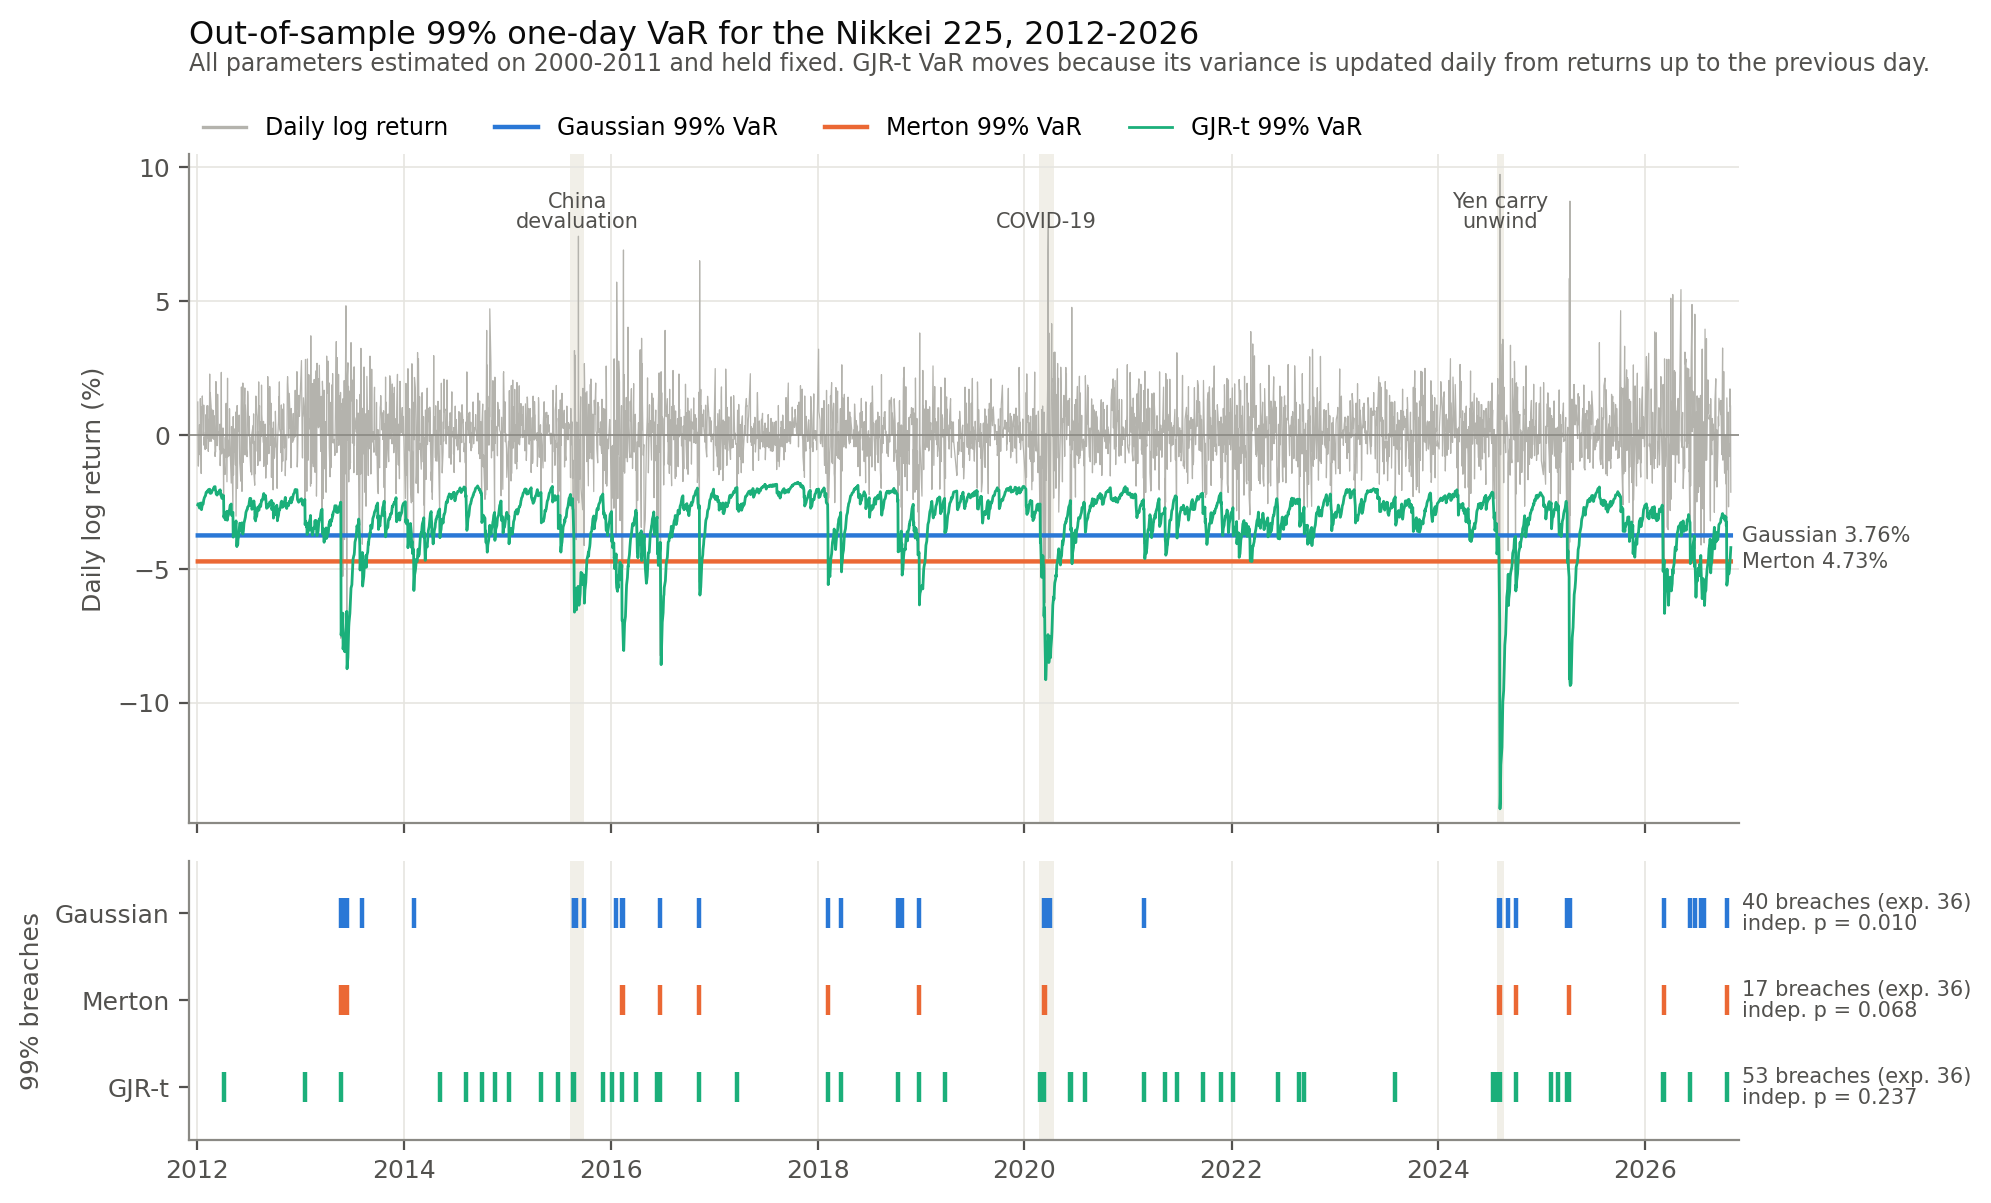
\includegraphics[width=0.88\textwidth]{var99_breaches.png}
\caption{Test-period returns with each model's 99\% VaR (top) and the dates of 99\% breaches (bottom). Shaded:
August--September 2015, February--April 2020 and late July--August 2024. Under GJR-$t$, breaches no longer follow one
another day after day, but crisis years still have more than their share: <<y2015>>, <<y2020>> and <<y2024>> breaches
in 2015, 2020 and 2024, against about <<y_exp>> expected per year. This is because the variance only rises after the
first large fall.}
\end{figure}

\section{Limitations}

All parameters come from a single 2000--2011 estimation and are never refitted. The test period is calmer than training
and has a higher mean (daily sd <<sd_te>>\% vs <<sd_tr>>\%, mean $<<mean_te>>\%$ vs $<<mean_tr>>\%$). Some of GJR-$t$'s
excess 99\% breaches may reflect stale parameters rather than the model form; an expanding-window refit was not tested.
There is one index, one split and one data source (Yahoo Finance, not cross-checked against an official series). Six
VaR models at three levels are tested, so a few rejections or passes are expected by chance, and the tests are not
adjusted for this. The model was chosen on training BIC. GARCH-$t$, which was not chosen, did better ex post at 99\%
(<<GT99_x>> breaches, $LR_{cc}$ $p = <<GT99_pcc>>$), but switching to it now would be selecting on the test set.
Christoffersen's test only detects day-to-day dependence, so it can pass while breaches still bunch within weeks, as in
Figure~1. Ljung--Box $p$-values on GARCH residuals use $h$ rather than $h-2$ degrees of freedom, the OLS $t$-statistics
ignore autocorrelation and heteroskedasticity, and the Merton density is truncated at 10 jumps.

\section{Conclusion}

Daily Nikkei returns are almost unpredictable in the mean, so VaR quality depends on the distribution.
\begin{itemize}
  \item \textbf{Fat tails alone (Merton)} improve the density fit, mainly near the centre, but give a VaR that is too
    conservative and still constant.
  \item \textbf{Volatility clustering} is the feature that fixes the Gaussian model's failure. GJR-$t$ raises the 99\%
    Christoffersen $p$ from <<G99_pind>> to <<J99_pind>> and passes every test at 95\%.
  \item \textbf{The extreme tail is not fixed.} With parameters fixed at 2000--2011 values, GJR-$t$ breaches too often at
    99\% and 99.5\%.
\end{itemize}
Next steps: an expanding-window refit for all three models, filtered historical simulation, a machine-learning
baseline, and USD/JPY or VIX as added explanatory variables.

\end{document}
